\documentclass{article}
\usepackage[utf8]{inputenc}
\usepackage{hyperref}
\usepackage{breakurl}
\usepackage{textcomp}
\usepackage{graphicx}
\usepackage[catalan]{babel}
\usepackage{subcaption}
\usepackage[a4paper,rmargin=1in,lmargin=1in]{geometry}
\usepackage{amsmath}
\usepackage[nottoc,numbib]{tocbibind}
\title{Crossy Road \\
		\large Videojocs 2017/18 Q1}
\author{David Hernàndez Morales}
\date{08/01/2018}

\begin{document}
\pagenumbering{gobble}
\maketitle
\newpage
\tableofcontents
\newpage
\pagenumbering{arabic}
\section{Crossy Road}
\subsection{Dades del joc}
El joc que s'intenta emular és Crossy Road \textsuperscript{\texttrademark}
publicat (i desenvolupat) el 20/11/2014 per \textit{Hipster Whale} \cite{webCrossy}
\cite{wikipediaCrossy}. A la figura \ref{logo} es pot veure el logo de Crossy Road
amb l'emblemàtic pollastre que pretèn donar resposta a la pregunta
\textit{Why did the chicken cross the road?} \cite{preguntaChicken}

\begin{figure}[h!]
	\includegraphics[width=\linewidth]{Logo.png}
	\caption{Logo del crossy road}
	\label{logo}
\end{figure}

Com es pot veure a la taula \ref{dadesSortida}, el primer llençament va ser en
\textit{iOS}. Amb \textit{Android} un mes després i \textit{Windows Phone}
quasi un any més tard. També hi ha una versió per \textit{tvOS}.

\begin{table}[h!]
	\begin{center}		
		\begin{tabular}{l|l}
		\textbf{Plataforma} & \textbf{Data de sortida} \\
		\hline
		iOS & 20 Novembre, 2014 \\
		Android & 23 Decembre, 2014 \\
		Windows Phone & 1 Maig, 2015 \\
		tvOS & 30 Octubre, 2015
		\end{tabular}
		\caption{Dates de sortida de Crossy Road.}
		\label{dadesSortida}
	\end{center}
\end{table}

\subsection{Mecàniques del joc i acollida}

L'objectiu del joc és avançar endavant evitant obstacles mòvils per la
carretera i utilitzant plataformes. A l'imatge \ref{inGame}
es pot veure el tipus d'obstacles que s'han de superar.
Té moltes similituds amb el joc de
Frogger \textsuperscript{\texttrademark}, fins al punt que ha sigut
descrit com un ``endless Frogger'' per la premsa \cite{endlessFrogger1}
\cite{endlessFrogger2}. La puntuació és el nombre de files superades i
el joc recorda el màxim al que has arribat. També hi ha monedes distribuïdes
per les diferents graelles. Quan el jugador triga molt en avançar, la càmera
el sobrepassa i una àguila l'atrapa. Per tant es marca des del principi molt
clarament l'objectiu. \newline

\begin{figure}
	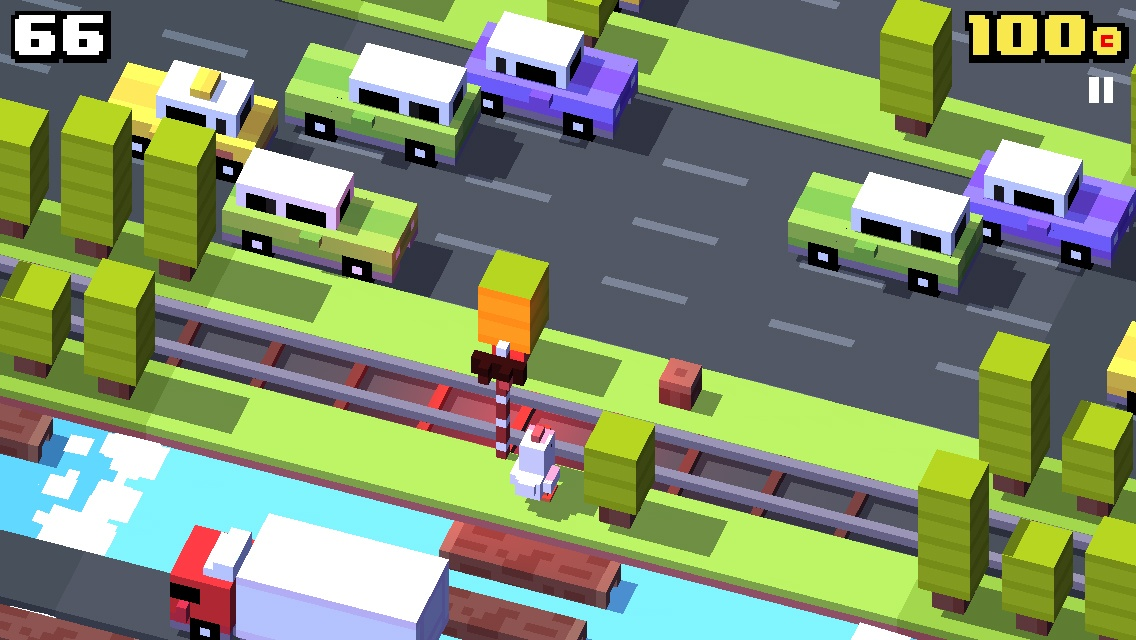
\includegraphics[width=\linewidth]{CrossyRoadGameplay.jpg}
	\caption{Imatge in-game de Crossy Road}
	\label{inGame}
\end{figure}

\subsection{Versions del joc}

Cal afegir que el joc va treure dues versions addicionals. Una versió de
Disney\textsuperscript{\textregistered} amb personatges com Mickey Mouse\textsuperscript{\texttrademark} i
Donald Duck\textsuperscript{\texttrademark} i amb altres personatges
de franquícies de Disney com The lion king\textsuperscript{\texttrademark}
o Toy story\textsuperscript{\texttrademark} \cite{disneyCrossy}. També,
donat l'èxit de Star Wars\textsuperscript{\texttrademark}, es va treure
una versió d'aquesta franquícia ja que era massa gran per incloure-la en
la de Disney \cite{starWarsCrossy}. \newline

\subsection{Desenvolupament}

Inicialment estava planejat dedicar només 6 setmanes al Crossy Road, però vist el
potencial del joc es va decidir dedicar sis setmanes més \cite{delayedCrossy}. L'equip
de \textit{Hipster Whale} és un equip independent composat per Andy Sum i Mat Hall, els
fundadors, l'artista Ben Weatherall i la presidenta Clara Reeves \cite{HipsterPressKit}.
Algunes tecnologies utilitzades pel joc són \textit{Qubicle} \cite{qubicle} \cite{crossyPressKit} o \textit{Unity}.

\subsection{Referències sobre el joc}

Algunes referències a tenir en compte a més de la web oficial \cite{webCrossy} són la wiki feta per
fans \cite{crossyWiki} amb els diferents enemics i/o personatges, el trailer
de google play \cite{trailerCrossy} o aquest gameplay que mostra la corva de dificultat
del joc \cite{gameplayCrossy}

\section{Descripció del projecte}

\subsection{Objectiu del joc}
Donat que el projecte intenta ser una còpia de \textit{Crossy Road}, els
objectius bàsics són els mateixos: avançar tant com es pugui sense morir i
superar la teva puntuació màxima. La puntuació és el nombre de files superades i
els enemics són els vehicles que es mouen per la carretera (cotxes, camions i trens)
i l'aigua, que és mortal. \newline

\subsection{Control i mecàniques}
Els controls són molt senzills. Amb les fletxes es mou el porc endavant, endarrere
i cap als costats. Així ho mostra la pantalla inicial del joc, com es mostra a la figura
\ref{menuInicial}, amb un dibuix de les fletxes. També es pot sortir del joc en
qualsevol moment amb el botó de ``exit game''.

\begin{figure}[h!]
	\includegraphics[width=\linewidth]{MenuInicial.png}
	\caption{Pantalla inicial del joc}
	\label{menuInicial}
\end{figure}

\subsubsection{Vehicles}

Com es mostra en la figura \ref{creuantCarretera}, mentre el jugador
creua per la carretera poden aparèixer cotxes, camions i fins i tot trens.
I tal i com apareix a la figura \ref{morintCarretera}, si no s'esquiven el personatge
mor, i surt la puntuació màxima que ha assolit fins al moment. També es dóna
l'opció de repetir el joc prement el botó de ``Play again''.

\begin{figure}[h!]
	\includegraphics[width=\linewidth]{CrossingStreet.png}
	\caption{Jugador creuant la carretera}
	\label{creuantCarretera}
\end{figure}

\begin{figure}[h!]
	\includegraphics[width=\linewidth]{DyingToVehicle.png}
	\caption{Jugador morint per un xoc}
	\label{morintCarretera}
\end{figure}

La densitat de vehicles ha estat evolucionant. Inicialment, es buscava
la densitat òptima de la següent forma: A cada frame i en una fila d'un
mateix sentit, es busca el cotxe més proper a l'origen de la fila.
Es calcul·la on interseccionaria amb un cotxe que fes spawn en aquell frame
amb la vel·locitat màxima. Si el punt de col·lisió és fora del punt
de despawn, llavors el cotxe fa spawn.
No obstant, això dóna una densitat de vehicles molt alta i el joc es
torna molt difícil. Per tant, s'introdueix un esbiaix que multiplica
el punt de despawn per a que sigui més difícil que un vehicle spawneji.
La fórmula és $\text{esbiaix} = 4 \cdot {1.1}^{-\text{filesAvançades}} + 1$.
D'aquesta forma la dificultat és més progressiva.

\subsubsection{Plataformes mòbils}

Com en el joc original, el personatge també ha de creuar plataformes mòbils.
Això es pot veure en la figura \ref{creuantAigua}. En aquest cas,
si el jugador es mou cap a un punt on hi hagi aigua, mor ofegat 
\ref{morintAigua}.

\begin{figure}[h!]
	\includegraphics[width=\linewidth]{CrossingWater.png}
	\caption{Jugador creuant l'aigua amb l'ajut dels troncs.}
	\label{creuantAigua}
\end{figure}

\begin{figure}[h!]
	\includegraphics[width=\linewidth]{DyingToWater.png}
	\caption{Jugador morint per ofec.}
	\label{morintAigua}
\end{figure}

En quant al disseny de les plataformes mòbils, hi havia un problema
afegit que els vehicles no tenien. I és que en el cas de les plataformes
mòbils, si no hi ha una certa coherència en la creació d'aquestes
es torna molt frustrant intentar creuar el riu. Es van pensar dues
estratègies:

\begin{enumerate}
	\item Tenir dos ``modes'' de spawneig. Lent i ràpid. Si una fila és
	ràpida la següent fila o bé és també ràpida i té el mateix sentit
	o bé és de sentit contrari. Si una fila és lenta no hi ha cap restricció.
	\item La fila següent és sempre de sentit contrari a l'anterior.
\end{enumerate}
En la pràctica, es va veure que el mètode 1 requereix molt de refinament perquè
si les velocitats són completament aleatòries (dintre d'un cert marge), es poden
crear buits en els que no hi ha cap forma de creuar el riu. Això passa quan
dos troncs tenen la mateixa velocitat i van en el mateix sentit però amb offsets
significatius. Per tant, tot i que simplifica més el joc,
es va acabar utilitzant la segona opció.

\subsubsection{Tren}

Un dels obstacles mòvils que també hi és present són els trens (veure figura 
\ref{trenPassant}). Aquest s'assemblen als vehicles normals però són més 
llargs, ocupant tota la pantalla i venen amb un canvi de model del senyal
i un so d'alerta. Aquests obstacles no tenen molta dificultat de disseny.

\begin{figure}[h!]
	\includegraphics[width=\linewidth]{TrainPassingBy.png}
	\caption{Tren passant}
	\label{trenPassant}
\end{figure}

\subsection{Menús}

En el joc original es pot canviar de personatge quan es mor o fins i tot 
descubrir personatges nous. Però, com que aquest joc està molt simplificat i només
hi ha un personatge, no hi ha un menú principal com a tal. Simplement
hi ha un botó per tonar a jugar quan mors i un slider pel volum del joc
i un botó per sortir del joc al principi. Es pot veure
a les imatges \ref{morintCarretera} i \ref{menuInicial}, respectivament.


\section{Metodologia}
El desenvolupament d'aquest projecte ha sigut una mica especial, ja que
al final he acabat presentant jo el projecte pel meu compte. Per tant,
donada la individualitat del projecte, no hi ha hagut reunions, ni fites, ni
diagrames de Gantt. Tampoc hi ha hagut sprints ni seguiment de
tasques mitjançant trello o slack perquè no tenia sentit sense
divisió de feina. \newline
Cal mencionar que en el joc 2D si que es va intentar utilitzar una metodologia
similar a la cascada ja que es va dissenyar el diagrama UML de les classes
bàsiques i després implementarles iterativament. No obstant, en aquest cas
com que el projecte és de Unity, no ho he vist necessari. \newline
La dedicació de temps al projecte també ha sigut una mica erràtica ja que al principi confiava
en que el meu company fes la seva feina. Amb el temps em vaig adonar de que
no seria així i, per tant, no hi ha hagut un diagrama de Gantt, sinó més bé
un sprint constant per arribar al deadline. El que si que s'ha utilitzat és un control de versions, més concretament git
amb github. El github del projecte es pot trobar a \cite{githubProjecte}.

\section{Conclusions}
El projecte ha sigut molt interessant. El meu objectiu personal respecte a
aquesta assignatura era conèixer com és un videojoc per dins.
Puc dir que, després d'acabar el projecte i conjuntament amb les classes de
teoria tinc una noció bàsica del que suposa el desenvolupament de videojocs.
No obstant, he de dir que m'agradaria fer un videojoc des de zero només
amb C++ i OpenGL per realment comprendre tots els aspectes.
Si hagués tingut un company de treball adient, potser no hauriem utilitzat
Unity i hauriem començat desde zero que és el que m'hauria agradat a mi.

\bibliography{Fonts}
\bibliographystyle{abbrv}
\end{document}
